\chapter{Implementation and Verification}
\label{chap:implementation}

\section{Programming Environment}
\label{sec:environment}

Implementation of the well-balanced method was carried out using the foam-extend 4.0 fork of the OpenFOAM (Open-Source Field Operation And Manipulation) software project. OpenFOAM was selected as it is a mature and feature rich platform for computational fluid dynamics, and thus already provides many utilities and functionality for tasks such as pre- and post-processing data, runtime selection of simulation parameters, and managing very generic meshes. It is coded entirely in object-oriented C++, making it also very flexible for extension.

The foam-extend fork was chosen over the standard OpenFOAM distribution as it includes an additional density-based Navier Stokes (DBNS) solver which implements very closely the basic FVM which was to be modified. As well, this DBNS library contains several already programmed numerical fluxes and gradient limiters, such that the focus could remain on developing the well-balanced reconstruction without having to code all of the supporting pieces from scratch.

For all of the simulations, the Rusanov flux~\cite{Rusanov1961} was chosen for the numeric flux function (i.e.\ the approximate Riemann Solver) and the Venkatakrishnan limiter~\cite{Venkatakrishnan1993,Venkatakrishnan1995} was used for the gradient limiting in the second order schemes. Both of these were used as already implemented in the DBNS library, with modifications only being made in the higher-level classes which called these modules, such that other limiter and flux function implementations could easily be swapped in if desired, using the runtime selectability provided by OpenFOAM.

The Rusanov flux was chosen as it inherently provided sufficient numerical dissipation to keep the simulations stable for all of the cases tested, while the HLLC and Roe flux functions, which are also implemented in the DBNS package, became unstable for the perturbed standing shock problem described in Section~\ref{subsec:sub_problem_2}.

The Venkatakrishnan limiter was chosen for its applicability to steady state flows, where the differentiability of its limiter function has been shown to speed convergence to stationary flow solutions. It is noted that some testing with the Barth-Jespersen limiter also produced satisfactory results for the convergence studies, and in general the choice of gradient limiter should not impact on the well-balanced nature of the scheme.

\subsection{Computational Time}
\label{subsec:timing}

As iterative Newton-Raphson solutions are required by the balanced scheme, this is expected to make it more computationally expensive than the standard methods for a given grid resolution. While the exact difference in compuational cost will depend on the memory requirements and set-up of the problem being simulated, a couple of CPU times are presented in Table~\ref{table:timing} for representative simulations in 1D, 2D, and 3D, to give an idea of the observed computational cost. These timings include initialization time and writing of final result files so they are only intended as a rough initial comparison between the unbalanced and well-balanced schemes.

\begin{table*}\centering
\caption{Computational times for sample problems in various dimensions comparing the second-order unbalanced and well-balanced schemes.}
\ra{1.3}
\label{table:timing}
\begin{tabular}{@{}crrrrrr@{}}\toprule
& \phantom{a} & \multicolumn{3}{c}{CPU time [$s$]} & \phantom{a} &\\
\cmidrule{3-5}
Dimension && unbalanced && well-balanced && Ratio\\ \midrule
1D && 313 && 1715 && 5.48\\
2D && 466 && 1999 && 4.29\\
3D && 17268 && 40386 && 2.34\\
\bottomrule
\end{tabular}
\end{table*}

It is noted that this work was primarily focused on the development, implementation, and testing of the new well-balanced method, not optimization thereof, so some level of improvement could almost certainly still be achieved over these results.


\section{Order Verification Study}
\label{sec:OVS}

An order verification study (OVS) was carried out to verify that the implementation matched the theoretically expected convergence rates. For the tests, a piecewise continuous potential function was defined on the 1D domain $x\in[-2,2]$, composed of two small constant regions at the boundaries connected by a fifth-order polynomial
\begin{equation}
\phi(x)=
\begin{dcases} 
      0, & x\leq -1.5 \\
      \frac{2}{81}x^5+\frac{5}{27}x^3+\frac{5}{8}x+\frac{1}{2}, & -1.5<x<1.5 \\
      1, & x\geq 1.5
\end{dcases}.
\end{equation}
The constant regions at the domain edges allowed for simple zero-gradient boundary conditions to be used for all non-fixed primitives, and the quintic coefficients were chosen to match also the first and second derivatives (to zero) at the transition points to the constant regions.

The inlet of the flow was set using dirichlet boundary conditions on $T$ and $v_x$ at $x=2$ with the values set to the same as those used for the inlet of sub-problem 1 described in Section~\ref{sec:TP_set_up} (see there for a more detailed description of how these values are determined). To briefly summarize here, at the inlet one has $p=0.75, T=1.05,$ and $v_x=-\sqrt{31/199}\approx-0.39$, with adiabatic constant $\gamma=4/3$ and units such that $c=\rho=1$. The inlet condition for the pressure is set to zero-gradient at the inlet, as having both it and the velocity fixed caused spurious error in some test cases and was recommended against in the OpenFOAM documenation. At the outlet, all primitives were given homogenous Neumann boundary conditions.

For the initial conditions in the rest of the domain, the value of the density $\rho(x)$ for a flow equilibrium flow was calculated, and then superimposed with a Gaussian perturbation centred at $x=0$, given by
\begin{equation}
\Delta \rho(x)=\frac{A}{2\sigma \sqrt{2 \pi}}\ \textrm{exp}\left[-\frac{1}{2}\left(\frac{x}{\sigma}\right)^2\right].
\end{equation}
The width of the Gaussian was determined with $\sigma=0.2$ and the amplitude $A$ was varied to control the maximal magnitude of the perturbation over several series of tests. Once the full $\rho(x)$ function was known, it was used to compute the other initial primitve values throughout the domain. In Fig.~\ref{fig:OVS_initial_profile} can be seen an example of these initial conditions as computed for the unperturbed equilibrium flow test.

\begin {figure}
\centering
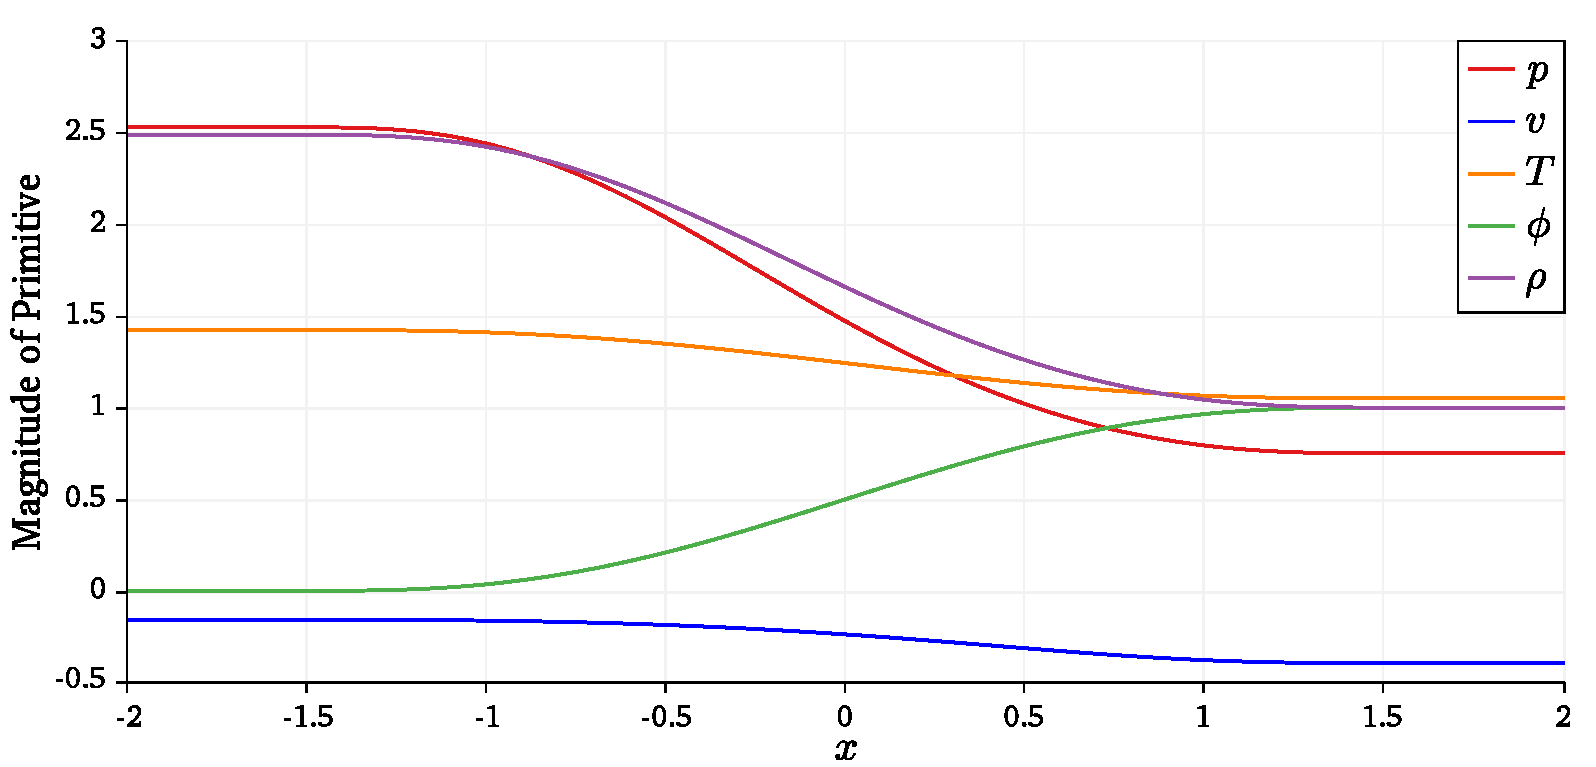
\includegraphics[width=13cm]{figures/OVS_initial_profile}
\caption {Magnitude profiles of the primitive values, density, and potential field at the initial time for the unperturbed equilibrium convergence test.}
\label{fig:OVS_initial_profile}
\end{figure}

Results of the simulations were characterized using the average absolute error magnitude, which is calculated as the normalized L1 norm of the error
\begin{equation} \label{eq:L1error}
Err_1=\frac{1}{N}\sum\limits_{i=1}^N \left|\rho_i-\rho_{i,\textrm{ref}}\right|,
\end{equation}
where $\rho_{\textrm{ref}}$ is a reference solution that is obtained either from exact calculation of the unperturbed equilibrium flow values, or from an overkill high-resolution simulation computed using $N=21870$ cells and the second-order well-balanced scheme for the test cases with the Gaussian perturbation. For the OVS, the number of cells is progressively tripled from $N=10$ to $N=7290$ and the intra-step order of accuracy is computed by determining the slope of the line connecting the error values of each adjacent pair of simulations using successively refined grids on a log-log plot of $Err_1$ vs.\ $\Delta x$.

Tripling was used such that when refining the grid, each cell would be perfectly split in three, and thus the position of the cell centre for the newly created middle cell would align exactly with the cell centre for the original coarse cell. Therefore, no interpolation is required to compare the cell centre values with the solutions obtained at any of the finer resolutions, and in particular the reference solution contains a value precisely at the location of each cell centre of every other grid resolution tested.

All convergence simulations were run to a final time of $t=1$, which was sufficient for the perturbations to have travelled significantly through the domain but still be most entirely contained within it.

\subsection{Equilibrium Flow}

The results of the first series of simulations at equilibrium, i.e.\ with $A=0$, are tabulated in Table~\ref{table:OVS_A0} and demonstrate very close agreement to the expected first- and second-order accuracy for the unbalanced schemes. For the well-balanced schemes, the average error is at the level of the machine precision for all grid resolutions, demonstrating the precise maintenence of the equilibrium flow irrespective of the number and size of the grid cells. This serves as a strong empirical verification of the precise matching between the source and flux term discretizations in the~\eqref{eq:balance} balance law for steady states, i.e.\ it truly is ``well-balanced''.

\begin{table*}\centering
\caption{L1 error of the density and intra-step order of accuracy for the first- and second-order unbalanced/well-balanced schemes with no perturbation, i.e.\ $A=0$.}
\ra{1.3}
\label{table:OVS_A0}
\begin{tabular}{@{}rcccccc@{}}\toprule
& \phantom{a} & \multicolumn{2}{c}{First} & \phantom{ab} & \multicolumn{2}{c}{Second}\\
\cmidrule{3-4} \cmidrule{6-7}
$N$ && $Err_1$ & Order && $Err_1$ & Order\\ \midrule
$10$ && 8.54e-02/4.04e-15 &&& 2.59e-02/4.04e-15 &\\
$30$ && 2.89e-02/5.20e-15 & 0.99/- && 3.16e-03/5.20e-15 & 1.91/-\\
$90$ && 9.77e-03/4.08e-15 & 0.99/- && 3.44e-04/4.09e-15 & 2.02/-\\
$270$ && 3.27e-03/3.63e-15 & 1.00/- && 3.77e-05/3.66e-15 & 2.01/-\\
$810$ && 1.09e-03/2.96e-15 & 1.00/- && 4.17e-06/5.05e-15 & 2.00/-\\
$2430$ && 3.64e-04/3.78e-14 & 1.00/- && 4.63e-07/5.20e-14 & 2.00/-\\
$7290$ && 1.21e-04/1.04e-14 & 1.00/- && 5.14e-08/1.37e-14 & 2.00/-\\
\bottomrule
\end{tabular}
\end{table*}

In Fig.~\ref{fig:OVS_A0} can be seen a visual representation of the same data from Table~\ref{table:OVS_A0}, making clear both the clean asymptotic convergence of the standard schemes as well as the many orders of magnitude greater accuracy achieved by the well-balanced method in simulating the stationary flow.

\begin {figure}
\centering
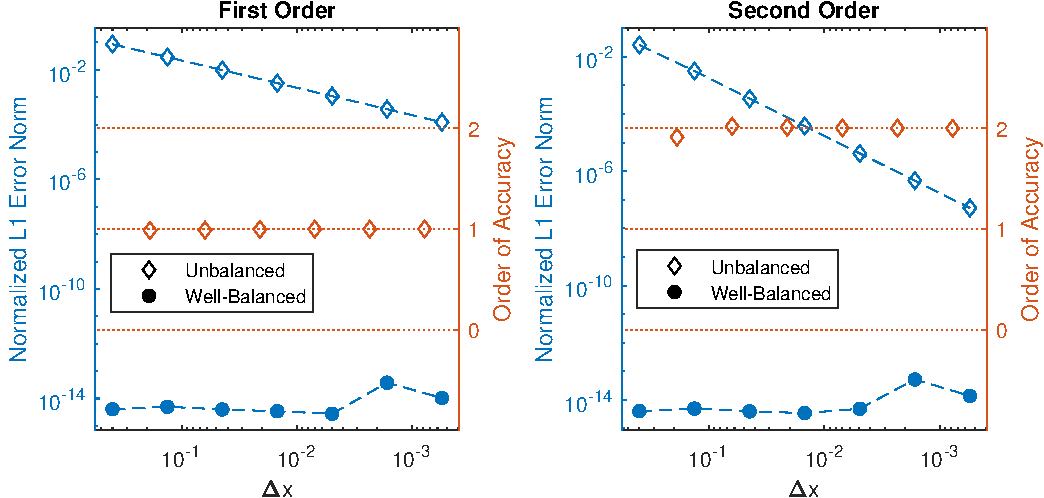
\includegraphics[width=13cm]{figures/OVSeps0}
\caption {L1 error of the density (in blue with dashed line) and intra-step order of accuracy (in red with no line) for the first- and second-order unbalanced and well-balanced schemes with no perturbation, i.e.\ $A=0$.}
\label{fig:OVS_A0}
\end{figure}

\subsection{Gaussian Perturbation}

Next is a series of tests using a `medium' amplitude Gaussian perturbation with $A=0.1$, with the initial and final density profiles of the reference solution shown in Fig.~\ref{fig:OVS_Amedium_profile}. This amplitude was chosen as it is large enough to be clearly resolved by all four combinations of first/second-order and un/well-balanced schemes, as seen in the table where all average errors are smaller than $A$. However, the amplitude was still small enough to ensure that the final solution remained smooth and does not yet present any steepening of flow features into discontinuities. Data from the convergence tests are presented in Table~\ref{table:OVS_Amedium} and visualized in Fig.~\ref{fig:OVS_Amedium}.

\begin {figure}
\centering
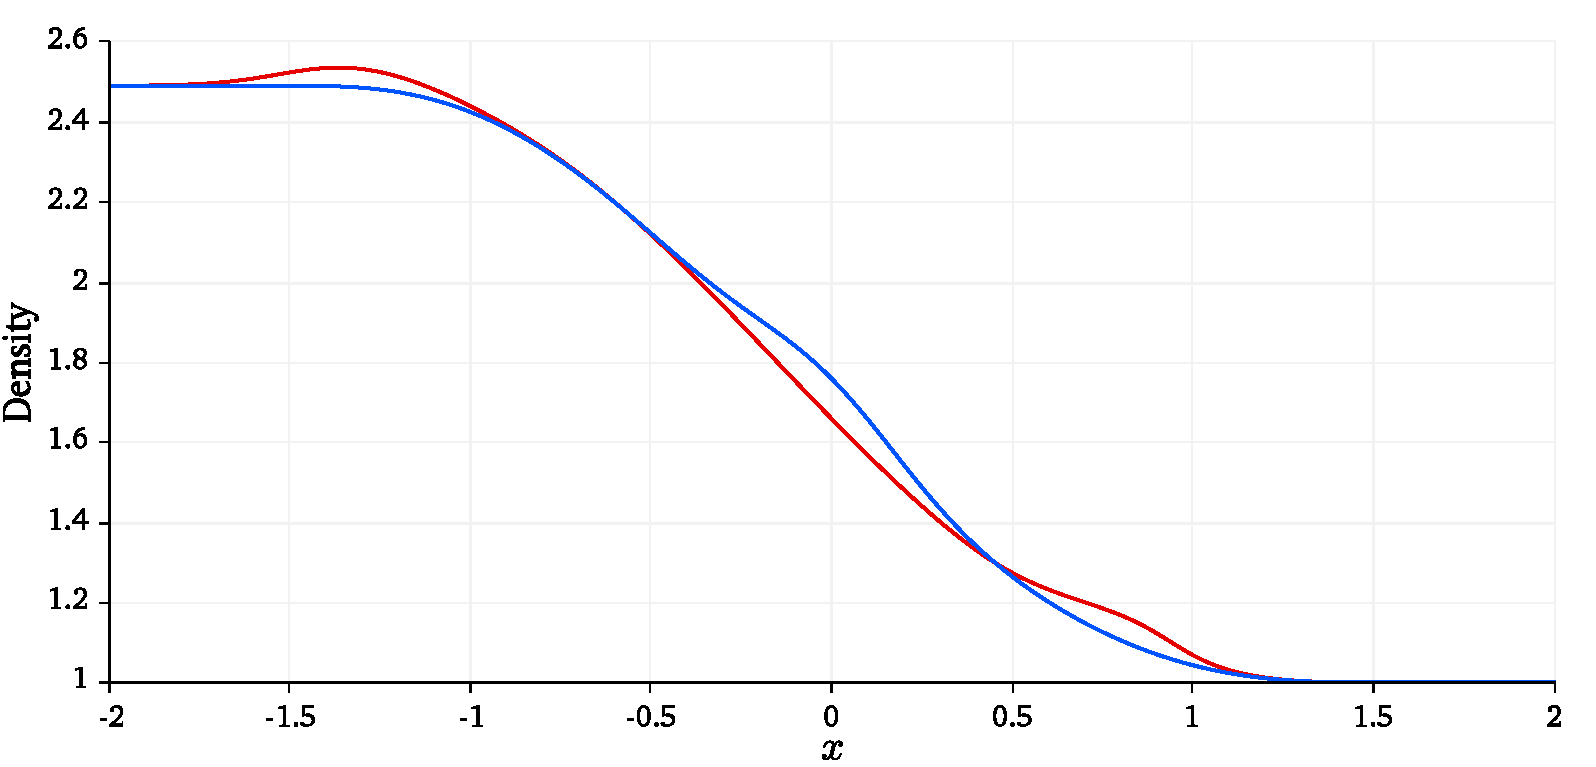
\includegraphics[width=13cm]{figures/OVSeps0_1profile}
\caption {Density profiles at the initial time (blue line) and final time (red line) of the reference simulation for the medium amplitiude $(A=0.1)$ convergence test, showing no discontinuities.}
\label{fig:OVS_Amedium_profile}
\end{figure}

It can be seen that the expected orders of accuracy are observed for the respective first- and second-order schemes where the graphs are in the asymptotic regime. In the second-order case it is noted that the results become abruptly non-linear for the smallest 1-2 grid spacings, due to the use of a reference solution which is itself only computed with the second-order well-balanced scheme using thrice as many cells as the final resolution presented on the plots. Thus the magnitude of errors still present in this reference becomes comparable to the errors in the final steps of the grid refinement, and so the linear convergence breaks down.

\begin{table*}\centering
\caption{L1 error of the density and intra-step order of accuracy for the first- and second-order unbalanced/well-balanced schemes with medium perturbation amplitude $A=0.1$.}
\ra{1.3}
\label{table:OVS_Amedium}
\begin{tabular}{@{}rcccccc@{}}\toprule
& \phantom{a} & \multicolumn{2}{c}{First} & \phantom{ab} & \multicolumn{2}{c}{Second}\\
\cmidrule{3-4} \cmidrule{6-7}
$N$ && $Err_1$ & Order && $Err_1$ & Order\\ \midrule
$10$ && 8.63e-02/1.23e-02 &&& 2.72e-02/7.51e-03 &\\
$30$ && 2.90e-02/9.68e-03 & 0.99/0.21 && 5.76e-03/3.78e-03 & 1.41/0.62\\
$90$ && 1.05e-02/5.63e-03 & 0.93/0.49 && 7.30e-04/5.29e-04 & 1.88/1.79\\
$270$ && 4.01e-03/2.61e-03 & 0.87/0.70 && 7.37e-05/5.34e-05 & 2.09/2.09\\
$810$ && 1.48e-03/1.01e-03 & 0.91/0.86 && 8.68e-06/5.89e-06 & 1.95/2.01\\
$2430$ && 5.14e-04/3.58e-04 & 0.96/0.95 && 2.97e-06/8.48e-07 & 0.98/1.76\\
$7290$ && 1.74e-04/1.22e-04 & 0.98/0.98 && 2.62e-06/5.80e-07 & 0.11/0.35\\
\bottomrule
\end{tabular}
\end{table*}

\begin {figure}
\centering
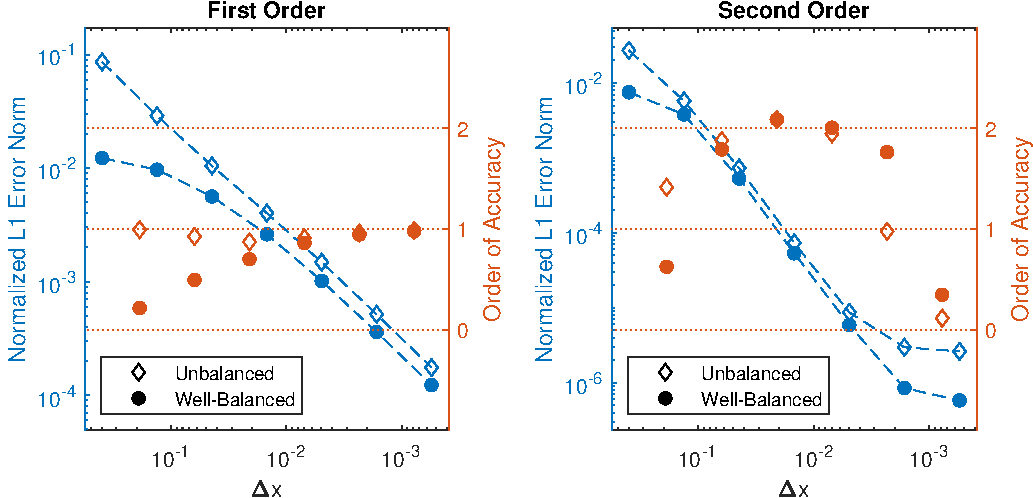
\includegraphics[width=13cm]{figures/OVSeps0_1}
\caption {L1 error of the density (in blue with dashed line) and intra-step order of accuracy (in red with no line) for the first- and second-order unbalanced and well-balanced schemes with medium perturbation amplitude $A=0.1$.}
\label{fig:OVS_Amedium}
\end{figure}

\subsection{Small Amplitude Perturbation}

In all cases for the medium amplitude, the well-balanced scheme is observed to have slightly lower errors than the unbalanced scheme, although the difference is relatively minor in this instance where the perturbation is much larger than the errors in the underlying equilibrium observed in the first convergence series with no perturbation. As such, we are interested in observing what happens for a perturbation amplitude that is quite small, comparable to or less than the average errors observed for the unbalanced scheme on the equilibrium flow. Therefore a third convergence series was carried out using a very small amplitude perturbation with $A=10^{-4}$, the results of which can be found in Table~\ref{table:OVS_Asmall} and Fig.~\ref{fig:OVS_Asmall}.

\begin{table*}\centering
\caption{L1 error of the density and intra-step order of accuracy for the first- and second-order unbalanced/well-balanced schemes with very small perturbation amplitude $A=10^{-4}$.}
\ra{1.3}
\label{table:OVS_Asmall}
\begin{tabular}{@{}rcccccc@{}}\toprule
& \phantom{a} & \multicolumn{2}{c}{First} & \phantom{ab} & \multicolumn{2}{c}{Second}\\
\cmidrule{3-4} \cmidrule{6-7}
$N$ && $Err_1$ & Order && $Err_1$ & Order\\ \midrule
$10$ && 8.54e-02/1.22e-05 &&& 2.59e-02/7.71e-06 &\\
$30$ && 2.89e-02/9.73e-06 & 0.99/0.21 && 3.17e-03/3.93e-06 & 1.91/0.61\\
$90$ && 9.77e-03/5.71e-06 & 0.99/0.49 && 3.44e-04/5.42e-07 & 2.02/1.80\\
$270$ && 3.27e-03/2.67e-06 & 1.00/0.69 && 3.77e-05/5.36e-08 & 2.01/2.11\\
$810$ && 1.09e-03/1.04e-06 & 1.00/0.86 && 4.17e-06/5.91e-09 & 2.00/2.01\\
$2430$ && 3.64e-04/3.67e-07 & 1.00/0.95 && 4.64e-07/8.39e-10 & 2.00/1.78\\
$7290$ && 1.21e-04/1.25e-07 & 1.00/0.98 && 5.28e-08/5.69e-10 & 1.98/0.35\\
\bottomrule
\end{tabular}
\end{table*}

\begin {figure}
\centering
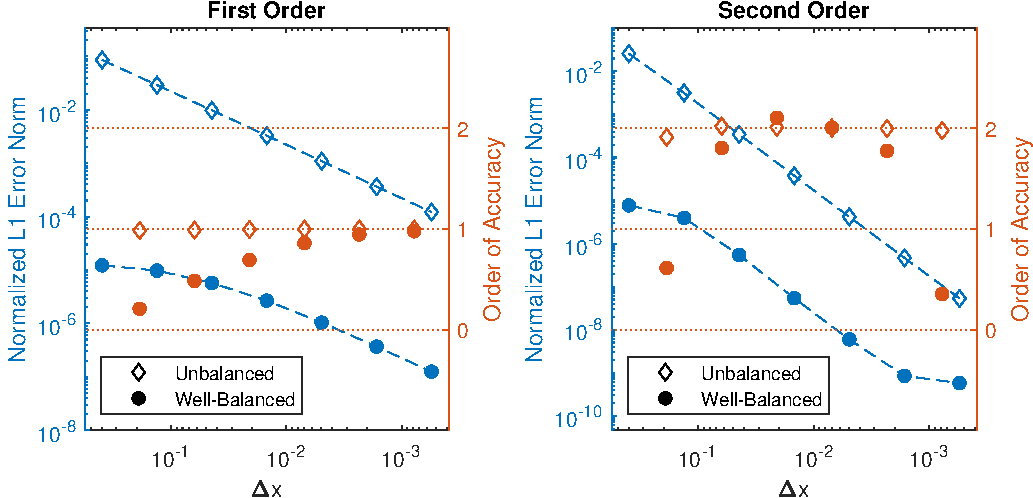
\includegraphics[width=13cm]{figures/OVSeps0_0001}
\caption {L1 error of the density (in blue with dashed line) and intra-step order of accuracy (in red with no line) for the first- and second-order unbalanced and well-balanced schemes with very small perturbation amplitude $A=10^{-4}$.}
\label{fig:OVS_Asmall}
\end{figure}

From the results, it is clear that the average error of the unbalanced scheme is much larger than the perturbation amplitude for all studied grid resolutions in the first-order case, and and even for the second-order scheme requires a fairly significant level of refinement before the error drops low enough for the perturbation to possibly be well resolved. The order of the convergence is of course still correct in both instances, but this is essentially just the same convergence towards the equilibrium as in the $A=0$ case, since the large magnitude of the errors compared to the perturbation amplitude mean that the deviation is not meaningfully percieved or simulated by the scheme over much of the parameter space.

By contrast, the well-balanced scheme exhibits average errors much smaller than the pertuabtion amplitude, with even the least resolved first-order simulation already having almost a full order of magnitude smaller error. Observed orders of convergence are the same as for the unbalanced scheme, but as exemplified visually in Fig.~\ref{fig:OVS_Asmall}, the absolute size of the errors is many orders of magnitude less for the well-balanced scheme. No level of grid refinement studied was able to get the first-order unbalanced scheme to the accuracy of its well-balanced counterpart, and it required approximately $3^3$ times more grid cells in the second-order tests to match the observed accuracy there. This demonstrates the potentially massive savings in computational cost provided by the well-balanced method for simulating small perturbations, especially in 2D or 3D simulations where the benefits would be compounded along each additional dimension.

\subsection{Discontinuous Flow}

Lastly, a large $A=2$ amplitude perturbation was used to investigate the performance of the schemes when steepened discontinuities become present in the solution. As seen in Fig.~\ref{fig:OVS_Alarge_profile}, the density profiles at the final time have developed clear discontinuities from the initially smooth profile. The results of the convergence tests for this amplitude are given in Table~\ref{table:OVS_Alarge} and reveal that the order of accuracy has now dropped to first-order for all schemes, because the gradient limiting means that the normally second-order schemes are reduced to first-order accuracy at the sharp transition points, and so this observed reduction in the convergence order agrees with the expected behaviour of such TVD limited reconstruction methods.

\begin {figure}
\centering
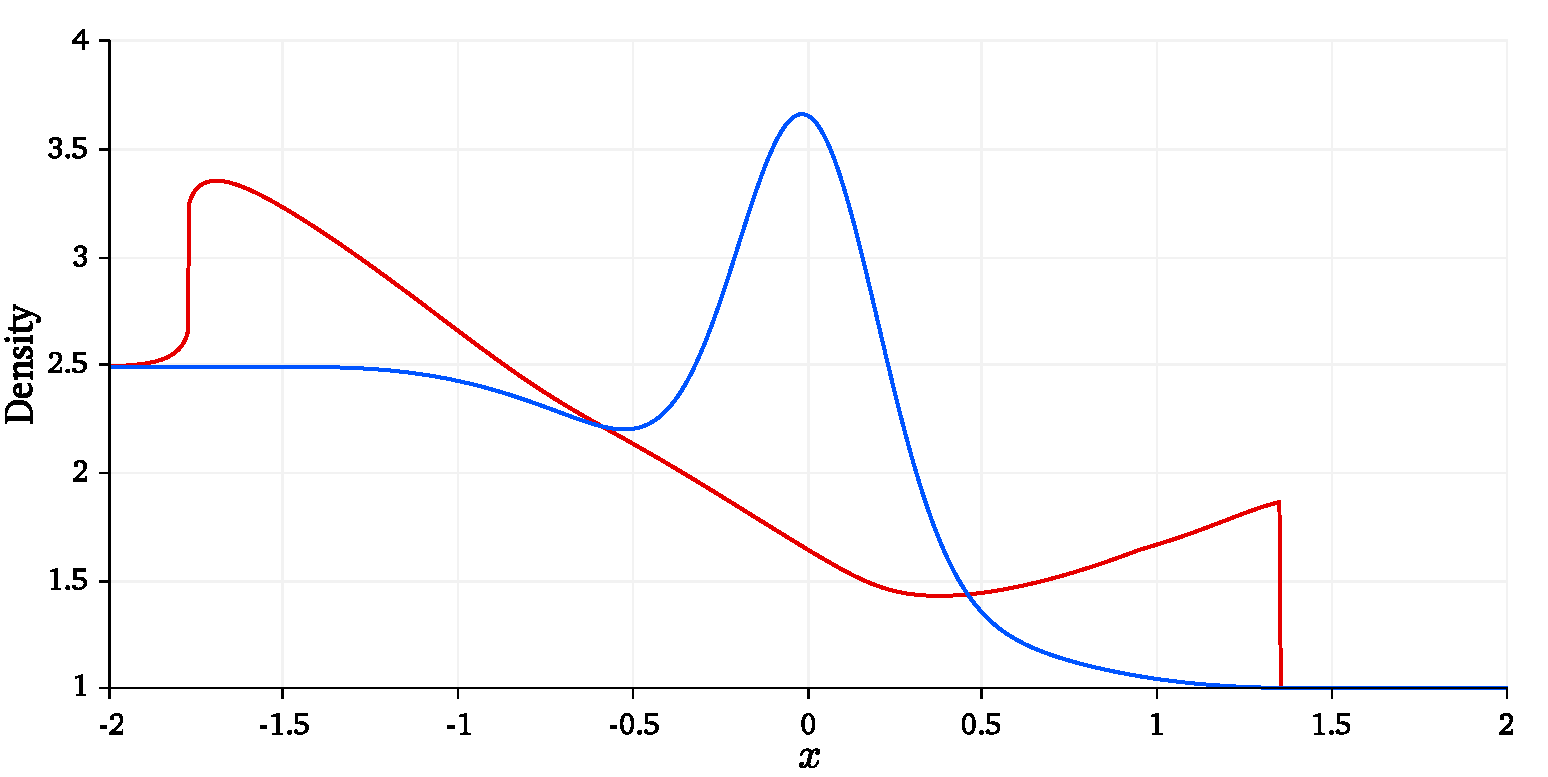
\includegraphics[width=13cm]{figures/OVSeps2profile}
\caption {Density profiles at the initial time (blue line) and final time (red line) of the reference simulation for the large amplitiude $(A=2)$ convergence test, showing clear discontinuities.}
\label{fig:OVS_Alarge_profile}
\end{figure}

Fig.~\ref{fig:OVS_Alarge} shows almost perfect overlap of the errors of the un/well-balanced schemes. As mentioned in Section~\ref{subsec:timing} the well-balanced scheme is more computationally expensive than the standard method for a given grid resolution, and combined with the earlier medium and small amplitude results, this implies that the use of the well-balanced scheme is only justified for simulations involving deviations from the equilibrium flow that are smaller than or comparable to the error in the equilibrium state for the standard scheme. For such cases, the machine precision accuracy of the equilibrium for the balanced scheme means the perturbation can be simulated with a (potentially much) coarser grid, thus countering the higher computational cost per cell to result in overall savings of required effort for a given level of accuracy.

\begin{table*}\centering
\caption{L1 error of the density and intra-step order of accuracy for the first- and second-order unbalanced/well-balanced schemes with very large perturbation amplitude $A=2$.}
\ra{1.3}
\label{table:OVS_Alarge}
\begin{tabular}{@{}rcccccc@{}}\toprule
& \phantom{a} & \multicolumn{2}{c}{First} & \phantom{ab} & \multicolumn{2}{c}{Second}\\
\cmidrule{3-4} \cmidrule{6-7}
$N$ && $Err_1$ & Order && $Err_1$ & Order\\ \midrule
$10$ && 2.12e-01/1.96e-01 &&& 1.13e-01/1.13e-01 &\\
$30$ && 1.43e-01/1.44e-01 & 0.36/0.28 && 5.06e-02/5.10e-02 & 0.74/0.73\\
$90$ && 8.04e-02/7.93e-02 & 0.52/0.54 && 1.75e-02/1.75e-02 & 0.97/0.97\\
$270$ && 3.69e-02/3.66e-02 & 0.71/0.70 && 5.26e-03/5.26e-03 & 1.09/1.10\\
$810$ && 1.50e-02/1.48e-02 & 0.82/0.83 && 1.88e-03/1.88e-03 & 0.94/0.93\\
$2430$ && 5.88e-03/5.80e-03 & 0.85/0.85 && 5.86e-04/5.82e-04 & 1.06/1.07\\
$7290$ && 2.18e-03/2.15e-03 & 0.90/0.90 && 2.00e-04/1.83e-04 & 0.98/1.05\\
\bottomrule
\end{tabular}
\end{table*}

\begin {figure}
\centering
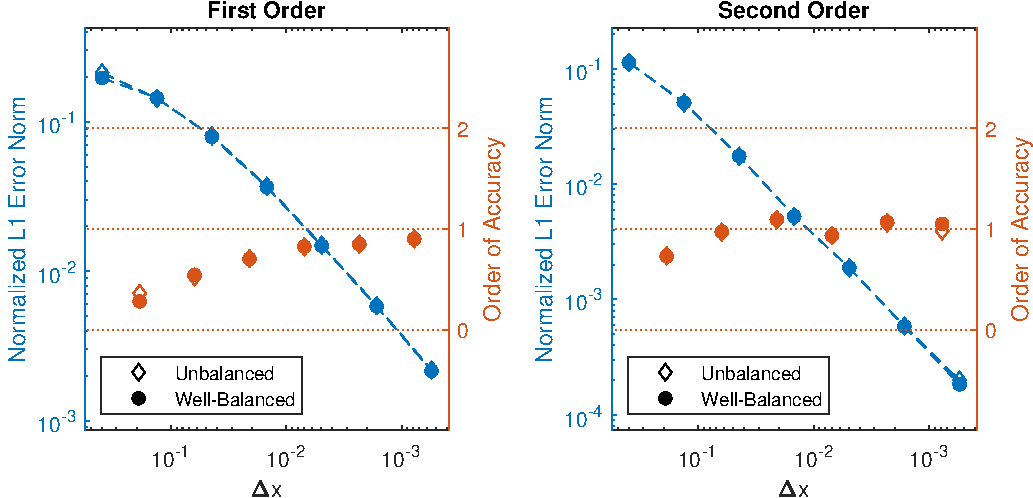
\includegraphics[width=13cm]{figures/OVSeps2}
\caption {L1 error of the density (in blue with dashed line) and intra-step order of accuracy (in red with no line) for the first- and second-order unbalanced and well-balanced schemes with large perturbation amplitude $A=2$.}
\label{fig:OVS_Alarge}
\end{figure}

For all amplitiudes, a good agreement is seen between the experimental results and the theoretically expected orders of accuracy, providing a solid verification of the correct implementation of the new well-balanced scheme.


\section{3D Polytrope}
\label{sec:polytrope}

With the formal accuracy now demonstrated for regular 1D gemoetries, a higher dimensional test is carried out using a simple astrophsyical problem. The 3D polytrope example from KM is chosen, to also illustrate the recovery of the hydrostatic case by the newly extended scheme. This problem simulates a hydrostatic configuration of adiabatic gases held together in a sphere by self-gravitation, according to the spherical equilibrium
\begin{equation} \label{eq:polyEquilibrium}
\frac{\textrm{d}p}{\textrm{d}r}=-\rho\frac{\textrm{d}\phi}{\textrm{d}r},
\end{equation}
and Poisson's equation in spherical symmetry
\begin{equation} \label{eq:spherePoisson}
\frac{1}{r^2}\frac{\textrm{d}}{\textrm{d}r}\left(r^2\frac{\textrm{d}\phi}{\textrm{d}r}\right)=4\pi G\rho,
\end{equation}
with the radial variable and gravitaitonal constant as $r$ and $G$, respectively.

Using the polytropic equation of state~\eqref{eq:polyEOS}, one can combine Eqs.~\eqref{eq:polyEquilibrium} and \eqref{eq:spherePoisson} into the single Lane-Emden equation
\begin{equation}
\frac{1}{r^2}\frac{\textrm{d}}{\textrm{d}r}\left(r^2\gamma K\frac{\textrm{d}\phi}{\textrm{d}r}\right)=-4\pi G\rho,
\end{equation}
which has analytic solutions for three adiabatic constants $(\gamma=6/5,2,\inf)$. $\gamma=2$ will therefore be used for the following tests, as neutron stars can be modeled by $\gamma\in[2,3]$ and an analytical solution exists.

This then gives the following analytic gravitational potential and primitive variable profiles
\begin{align}
\phi(r)&=-2K\rho_c\frac{\sin(\alpha r)}{\alpha r}, \\
\rho(r)&=\rho_c\frac{\sin(\alpha r)}{\alpha r}, \\
p(r)&=K\left(\rho_c\frac{\sin(\alpha r)}{\alpha r}\right)^2, \\
T(r)&=\frac{K\rho_c}{R}\frac{\sin(\alpha r)}{\alpha r},
\end{align}
where $\rho_c$ is the density at the centre of the polytrope, $R$ is the specific gas constant, and
\begin{equation}
\alpha=\sqrt{\frac{4\pi G}{2K}}.
\end{equation}

Note that the configuration is hydrostatic so the velocity profile is simply $v(r)=0$ everywhere. The model constants are set as $K=G=\rho_c=1$ and $R=5/7$.

The polytrope was simulated over a spherical domain of radius $0.5$ centred at the origin. Unstructured tetrahedral meshes with varying numbers of cells $N$ were generated using the Delauney algorithm of Gmsh, followed by mesh optimization with both the standard Gmsh and Netgen optpimizers in the Gmsh package.  Initial field profiles were simply set using the analytic solutions. Dirichlet boundary conditions were used for all fields exept the velocity, and were fixed to the analytic values, with the velocity then given a homogenous Neumann boundary condition.

Results of the simulations are given in Table~\ref{table:polytrope}, again using the L1 error norm~\eqref{eq:L1error} of the density to characterize the deviation from the analytic equilibrium. All simulations were run to a final time $t=1$ with a timestep $\Delta t=0.001$ for a total of $1000$ timesteps. Measuring the spatial order of accuracy for an unstructured mesh is a much complicated problem than for a regular cartesian grid, as each cell can have it's own size and shape. Therefore a characteristic length scale must be specified for each tested mesh, in order to approximate the order of accuracy for the convergence of the solutions.

\begin{table*}\centering
\caption{L1 error of the density and approximate intra-step order of accuracy for the first- and second-order unbalanced/well-balanced schemes for 3D polytrope on $N$ cell tetrahedral mesh.}
\ra{1.3}
\label{table:polytrope}
\begin{tabular}{@{}rlccccc@{}}\toprule
&& \multicolumn{2}{c}{First} &  & \multicolumn{2}{c}{Second}\\
\cmidrule{3-4} \cmidrule{6-7}
$N$ & \phantom{al}$h$ & $Err_1$ & Order && $Err_1$ & Order\\ \midrule
$4144$ & 0.585\phantom{a} & 8.17e-03/1.23e-15 &&& 4.22e-04/1.31e-15 &\\
$28036$ & 0.327 & 6.02e-03/1.22e-15 & 0.54/- && 2.06e-04/1.29e-15 & 1.24/-\\
$233064$ & 0.177 & 3.54e-03/1.23e-15 & 0.87/- && 1.07e-04/1.37e-15 & 1.07/-\\
$1857454$ & 0.097 & 1.94e-03/1.24e-15 & 1.01/- && 6.04e-05/1.99e-15 & 0.96/-\\
\bottomrule
\end{tabular}
\end{table*}

In this study, such a characteristic length, denoted $h$, was computed by using the volume of the largest mesh cell to determine the side length of a regular tetrahedron of that volume, with that side length then multiplied by the largest aspect ratio of the cells in the mesh. It is noted that this $h$ is not intended to represent an actual physical length in the mesh, but to provide a single metric which takes into account both the size and quality of the cells present in the mesh, and which should scale comparably between meshes generated using the same algorithm.

Analyzing the results revealed only machine precision deviation from the analytic equilibrium for the first- and second-order new schemes on all mesh sizes, confirming the well-balanced properties even on an unstructured tetrahedral mesh. The standard scheme, by contrast, produces spurious perturbations, which do converge to the analytic solution with increasing mesh resolution. For the first-order scheme, the approximate order of accuracy approaches the expected value of $1$ as the mesh is refined, while for the second-order scheme the order actually decreases towards $1$ as well for higher $N$, although the magnitude of the error is lower than for the first order scheme.

Some of this deviation may be due to the approximate nature of the characteristic length used for the analysis, but it has also been shown by Roe~\cite{Roe1987} that local truncation error for some FVMs is only first-order accurate for very irregular triangular meshes. Therefore this first-order accuracy on tetrahedral meshes meshes may not be entirely surprising, although Lindquist and Giles~\cite{Lindquist1989} and Giles~\cite{Giles1989} have shown that for some triangular meshes global second-order accuracy is possible, so perhaps for a higher-quality and more precise characteristic length a better convergence order could be demonstrated. However, as the well-balanced schemes, not the standard schemes, are the focus of this thesis, such further studies are not undertaken here.
